
\documentclass{beamer}
\usepackage{rtrees}
\usepackage{tree-dvips,url}
%\usepackage{qtree}
\usepackage{beamerthemetree}
%\usepackage{beamerthemesplit}
\usepackage{color}
\usepackage{lingmacros}
\setbeamertemplate{footline}[frame number]
\usepackage{graphicx}
%\usepackage{xyling}
%\usepackage[swedish]{babel} 
\usepackage[latin1]{inputenc} 
\usepackage{egapa,avm}
\newcommand{\newblock}{}
\newcommand{\mq}{MaxQUD }
\newcommand{\whp}{WhP }
\newcommand{\fe}{FEC }
\usepackage{hyperref}


\title{Introduction to  Semantics with Type Theory with Records for Natural Language:\\
  Lecture 5     }
\author{Jonathan Ginzburg\\
Universit\'e Paris-Diderot, Sorbonne Paris-Cit\'e\\
Robin Cooper\\ 
University of Gothenburg}
\date{}

\AtBeginSection[]
{
   \begin{frame}[plain]
       \frametitle{Outline}
       \tableofcontents[currentsection]
   \end{frame}
}

\newcommand{\backgroundyellow}{\beamertemplateshadingbackground{yellow!40}{magenta!20}}
\newcommand{\backgroundwhite}{\beamertemplateshadingbackground{white!100}{white!100}}
\newcommand{\ba}{\begin{avm}}
\newcommand{\ea}{\end{avm}}


\newenvironment{display}{\begin{center}}{\end{center}}

%
% Reference the next example in the text:
%
\newcommand{\nexteg}[1]{\addtocounter{examplectr}{1}(\arabic{examplectr}{#1})\addtocounter{examplectr}{-1}}
%
% Reference the previous example in the text:
%
\newcommand{\preveg}[1]{(\arabic{examplectr}{#1})}
%
% Reference examples by relative offsets:
%
\newcommand{\egnum}[2]{\addtocounter{examplectr}{#1}(\arabic{examplectr}{#2})\addtocounter{examplectr}{-#1}}
%
%
% ENVIRONMENTS
%
% Examples Environments
%
\newcounter{examplectr}
\newcounter{subexamplectr}[examplectr]
\renewcommand{\thesubexamplectr}{\alph{subexamplectr}}
%
% Sub-example Macro:
%
\newenvironment{subex}%
   {%\vspace*{-.8\baselineskip}
     \begin{list}
       {\alph{subexamplectr}.}%
       {\setlength{\topsep}{0in}
        \setlength{\leftmargin}{1em}%{0.25in}
        %\setlength{\listparindent}{-2em}
        %\setlength{\labelsep}{\baselineskip}
 \usecounter{subexamplectr} }
       }%
   {\end{list}}
%
% Single Example Macro
%
% \newenvironment{ex}%
%    { \refstepcounter{examplectr}
     
% \bigskip

%     % \begin{list}
%       % {
%        (\arabic{examplectr})%}%
%        % {%\setlength{\topsep}{0in}
% %         \setlength{\leftmargin}{4em}%{0.75in}
% %         \setlength{\labelsep}{\baselineskip}
% % }
%         \hspace*{1em}\begin{minipage}[t]{4in} 
% %\item
%    }%
%    {\end{minipage}

% \bigskip

%     %\end{list}
% }
% %
% % End of example macro
% %
\newcommand{\bit}{\begin{itemize}}
\newcommand{\eit}{\end{itemize}}
\newcommand{\ben}{\begin{enumerate}}
\newcommand{\een}{\end{enumerate}}
\newcommand{\ignore}[1]{}
\newcommand{\eeen}{\eenumsentence}
\newcommand{\subegref}[2]{(\ref{#1}\ref{#2})}

%\newcommand{\beg}{\begin{ex}}
%\newcommand{\eeg}{\end{ex}}
%\newcommand{\bseg}{\begin{subex}}
%\newcommand{\eseg}{\end{subex}}


\newcommand{\egstack}[1]{\begin{tabular}[t]{@{}l@{}} #1 \\ \\
  \end{tabular}}

%Records

\newcommand{\record}[1]{$\left[\mbox{\begin{tabular}{lcl} #1
\end{tabular}}\right]$} 
\newcommand{\smallrecord}[1]{$\left[\mbox{\begin{tabular}{@{}l@{}c@{}l@{}} #1
\end{tabular}}\right]$}

\newcommand{\field}[2]{#1 & = & #2}
\newcommand{\tfield}[2]{#1 & : & #2}
\newcommand{\smalltfield}[2]{#1:#2 & &}
\newcommand{\mfield}[3]{#1=#2 & : & #3}
\newcommand{\smallmfield}[3]{#1=#2:#3 & &}
\newcommand{\hfield}[2]{{\sc #1} & & #2}




\begin{document}
\maketitle


\ignore{
Lecture 4.
We provide a unified theory of metacommunicative and illocutionary interaction on the basis of the notion of Austinian locutionary propositions. This provides a basis for describing various linguistic phenomena occuring during grounding and clarification interaction.
}

\frame[plain]{\frametitle{Outline}\tableofcontents}


\section{NSUs}

\frame{
Based on \cite{ginzburg-buke}, Chapter 7 (on the website).
}


\begin{frame}\frametitle{A corpus study of NSUs}

\begin{itemize}

\item Corpus study of NSUs in the BNC
  (\cite{fernandez-ginzburg-tal,raquel-diss}). A randomly selected
  section of 200-speaker-turns from 54 BNC files.  The examined
  sub-corpus contains 14,315 sentences.


\item A total of 1299 NSUs were found.  Of these, 1283 were labelled
  according to a typology described below, the remaining 16 instances
  did not fall in any of the categories of the taxonomy.

\ignore{
\item 
The labelling of the entire corpus of NSUs was done by one expert
annotator.

\item Two additional, non-expert annotators
annotated a total of 50 randomly selected instances  with the classes in the taxonomy.  


\item  $\kappa$:  0.76.  The non-expert annotators
  also achieved 92 \% and 96\% in antecedent sentence identification
  for each NSU, relative to expert annotation as a gold standard.}
  \end{itemize}\end{frame}



\begin{frame}\frametitle{NSUs: some corpus data}

{\tiny
\begin{center}
\begin{tabular}{|lc||c||c||}\hline
{\bf NSU class}       &  {\bf Example} & {\bf Total} \\\hline
Plain Acknowledgement & \emph{A: \ldots B: mmh} & 599 \\
Short Answer    & \emph{A: Who left? B: Bo}      & 188 \\
Affirmative Answer  & \emph{A: Did Bo leave? B: Yes}  & 105 \\
C(larification) E(llipsis) &          \emph{   A: Did Bo leave? B:
  Bo?} &\\
Reprise sluices & \emph{A: Did Bo Leave? B: Who?}   & 92 \\
Repeated Ack. & \emph{A: Did Bo leave? B: Bo, hmm. }  & 86 \\
Rejection    &  \emph{ A: Did Bo leave? B: No. }     & 49 \\
Factual Modifier  &  \emph{ A: Bo left. B:  Great! }   & 27 \\
Repeated Aff. Ans.  & \emph{ A: Did Bo leave? B: Bo, yes. }   & 26 \\
Helpful Rejection     & \emph{ A: Did Bo leave? B: No, Max. } & 24 \\
Check question & \emph{A: I'm coming. Okay?} & 22 \\
Filler    & \emph{ A: Did Bo \ldots B: leave? }             & 18 \\
Bare Mod. Phrase &   \emph{ A: Max left. B: Yesterday. }   & 15 \\
Propositional Modifier & \emph{ A: Did Bo leave? B: Maybe. } &11 \\
Direct Sluice         & \emph{ A: Someone left. B: Who? }        & 11 \\
Conjunction + frag    & \emph{ A:  Bo left. B: And Max. } &10  \\
Other & & 16\\
\hline
{\bf Total dataset}  & & {\bf 1109}\\ \hline
\end{tabular}

\textbf{Table 2: BNC NSU corpus study } 

\end{center}
}
\end{frame}

\frame{\frametitle{Which classes can we already describe?}

}


\begin{frame}\frametitle{Yes}

\bit
\item  treat `yes' as an  adverb
 (English: intransitive, IC[+]) 

\eenumsentence{\label{yes1}\item[]
\begin{avm}
\avml\[
{\sc phon} : {\tt yes }\\
{\sc cat} = {\it adv[+ic]} : syncat\\
%{\sc arg-st} = \< \ \> : elist(synsem)\\
{\sc dgb-params.max-qud} : PolQuestion\\
{\sc cont} = max-qud(\[ \ \]): Prop \\
   \]\avmr
\end{avm}
}
\eit
\end{frame}

\frame{\frametitle{Right?}
\eeen{\item[]
\begin{avm}
\avml\[
phon : {\tt right }\\
cat.head = interj : syncat\\
%{\sc arg-st} = \< \ \> : elist(synsem)\\
dgb-params : \[spkr : IND\\
                             addr : IND\\
                             utt-time : TIME\\
                             LatestMove.content =\\   Assert(spkr,addr,p) : IllocProp\\
\]\\
cont = Check(spkr,addr,utt-time,p?) : IllocProp \\
   \]\avmr
\end{avm}}
}

\frame{\frametitle{Really?}
\eeen{\item[]

\begin{avm}
\avml\[
phon : {\tt really }\\
cat.head = interj : syncat\\
%{\sc arg-st} = \< \ \> : elist(synsem)\\
dgb-params : \[spkr : IND\\
                             addr : IND\\
                             utt-time : TIME\\
                             LatestMove.content = \\  Assert(addr,spkr,p) : IllocProp\\
\]\\
cont = Doubt(spkr,addr,utt-time,p?) : IllocProp \\
   \]\avmr
\end{avm}}

}

\frame{\frametitle{What remains to be done?}

\bit

\item partial parallelism: short answers, direct sluicing

\item metacommunicative NSUs

\item Genre dependent NSUs
\eit

}

\frame[allowframebreaks]{\frametitle{Sententialism v.\ Dialogue oriented constructionism}

\bit

\item
How should NSUs be incorporated in grammatical analysis? 

\item 
This depends to a large extent on 
%how one resolves the issue of 
whether NSUs are to be assimilated to another grammatical phenomenon
such as phonological reduction or anaphora. (See e.g.\   for sluicing    \cite{ross69,clm95,merchant02}, for short answers  \cite{morgan73,merchant04}.)

\item 
In theories that follow this route ({\it unitarian} theories), ellipsis resolution is associated with a single, typically extra-grammatical mechanism.

\item  
Alternatively, NSUs are in some significant way {\it sui generis}: in {\it constructionist} theories, NSUs are incorporated in the grammar as distinct constructions which specify a.o.\ the contextual characteristics which govern their use.

\item Extensive argumentation against underlying sententialism in (\cite{gs00,stainton-nsubook,nykiel2011remarks,ginzburg-buke})
based on:
\bit

\item Syntactic and semantic mismatches between NSU and reconstruction
  correlate.
\item Contextual explicitness.
\item Language acquisition: acquisition of NSUs is a long drawn out
  process of $>$ 2 years with various types of NSUs unexpectedly
  delayed relative to uniformity expectation of sententialism
  (\cite{gk-jl08}, Kolliakou and Ginzburg, 2012) 

\eit
\eit






}

\begin{frame}\frametitle{Focus establishing constituents}

\bit

\item In all the cases we have considered so far, the NSU can be described
completely on the basis of the fragment's own grammatical
characteristics and \mq  ({\sc max-pending} in the case of acknowledgements.).

\item One additional contextual parameter to track,
an antecedent sub-utterance (of utterance which is {\sc max-qud}).

\item
 Intuitively, this parameter provides a partial
specification of the focal (sub)utterance, and hence it is dubbed the
{\it focus establishing constituent} (FEC) 

\item  Varying roles played by the
FEC: in some cases it is crucial for the semantic composition, in
others it plays a disambiguating role via morphosyntactic or
phonological parallelism.
\eit
\end{frame}

\begin{frame}\frametitle{Focus establishing constituents}

\bit
\item Direct
sluicing involves in essence building a question whose domain derives
from the fragment whP and whose range derives from \mq :

\eeen{\label{sem-dep1}
\item A: A student complained about one of our teachers.\\
B: Who?
}

\item Content of \mq  after A's utterance 


                    {\footnotesize    \ba(\[ \])\[x : Ind\\
                            c1 : student(x)\\ 
                             y : Ind\\
                             c2 : teacher(y) $\wedge$ possess(w,y)\\ 
                            c0 : complain(x,y)\]\ea}

\item quest-dom of the whP: {\footnotesize \ba\[z : Ind\\
                                             c1 : person(z)\]\ea }

\item  We need to abstract over the index associated with a \whp, in
(\ex{1}c) the index $z$. 

\item This abstraction needs to be linked to a role
indexed by an antecedent NP, in this case $x$ or $y$. 

\eit\end{frame}

\begin{frame}\frametitle{Focus establishing constituents}

\bit
\item If no
identification of $z$ with $x$ or $y$ happens, the resultant content
will be as in (\ex{1}a), whereas what we desire is (\ex{1}b):

\eeen{
\item {\footnotesize \ba(r : \[z : Ind\\
                  c1 : person(z)\])\[x : Ind\\
                            c1 : student(x)\\ 
                             y : Ind\\
                             c2 : teacher(y) $\wedge$ possess(w,y)\\ 
                            c0 : complain(x,y)\]\ea}

\item {\footnotesize \ba(r : \[z : Ind\\
                  c1 : person(z)\])\[x = r.z : Ind\\
                            c1 : student(x)\\ 
                             y : Ind\\
                             c2 : teacher(y) $\wedge$ possess(w,y)\\ 
                            c0 : complain(x,y)\]\ea}
}
\eit
\end{frame}

\begin{frame}\frametitle{Focus establishing constituents}

\bit
\item 
For sluicing, in parallel with this semantic dependency comes a
syntactic dependency: Ross, 1969 pointed out, with reference to German,
that the fragment must concord to the case requirements of the
antecedent NP. 

\item Similar facts hold in various other languages where
case is overtly expressed, as documented in detail in
Merchant 2002

{\scriptsize
\eenumsentence{\label{roskas} \item
\shortex{9}{Er & will & jemandem  & schmeicheln,  & aber  & sie  &wissen  & 
nicht  & wem/{\#}wen.} 
{He  &wants  &someone-dat & flatter,  & but  & they 
&know  &not  &who-dat/{\#}who-acc.}
{He wants to flatter someone, but they don't know whom.}
\item 

\shortex{9}{Er  & will  &jemanden  &loben,  &aber  &sie  &wissen  &nicht 
&wen/{\#}wem.} 
{He & wants & someone-acc & praise, & but  &they  &know  &not 
&who-acc/{\#}who-dat.}
{He wants to praise someone, but they don't know whom.}
}}
\eit
\end{frame}

\begin{frame}\frametitle{Focus establishing constituents}

\bit

\item
There are a number of NSU types where a syntactic dependency exists
between an antecedent and the fragment, without there being a semantic
dependency above and beyond what \mq encodes already:
  
\eenumsentence{\label{greek-ex}
\item \shortex{5}{ A:  & lemi  &hixmeta?  & B: & {\#}moti/lemoti.}
{ & To-who  &flattered-2nd-sg?  &  & moti/to-moti}
{A: Who did you flatter? B: Moti. }

\item \shortex{7}{ A:  & et  &mi  & \v{s}ibaxt? & B:  &et  &moti/{\#}lemoti.}
{ & def-acc  & who  & praised-2nd-sg? &  & def-acc  & moti/to-moti}
{A: Who did you praise? B: Moti.}
}

\item CE$_{intended-content}$ constitutes perhaps the most extreme
  case of parallelism, since it involves segmental phonological
  parallelism with the source:

\eenumsentence{
\item[(i)] A: Did Bo leave? B: Max? (cannot mean: 
intended content reading: {\bf Who are you referring to?} )

 }
\eit
\end{frame}

\ignore{
\begin{frame}\frametitle{Semantic without syntactic parallelism}
\bit
\item Exclams constitute an NSU type in which there is a purely semantic dependency
between an antecedent sub-utterance and the NSU; the antecedent
supplies the referent of which the property encoded in the whP predicates:

 \eeen{\item \  A: Hercules cleaned the Augean stables.

B1: What a hero (Hercules) \ignore{$\mapsto$ \ba\[h : Ind\\
                                                                 c1 :
                                                                 unusual(hero(h))\\
                                                                   \]\ea  }

B2: What a terrible task (to clean the Augean stables).

B3: What a horrible place (the Augean stables were).
\ignore{$\mapsto$ \ba\[a : Ind\\
                                                                 c1 : unusual(horrible)(a)\]\ea  }
}
\item Even in languages where case is clearly
marked, exclams do not exhibit categorial concord with their
antecedents. 
\item This is illustrated in the Hebrew example in (\ex{1}), where
the noun `haoto' bears accusative case in the antecedent but not in the
exclam:

\eenumsentence{\item[] 
\begin{tabular}{rrrrr}
A:& natati & et-haoto& le-Moti.\\
 A:& gave-1st-sg &the-car(acc)& to Moti.\\
B:& &eyzo& gruta'a!\\
 B:& &What-a(nom)& wreck! 
\end{tabular}
}
\eit\end{frame}
}

\begin{frame}\frametitle{Focus establishing constituents}

\bit
%\item  What of the disapearance of \fe's? Here
%the simplest hypothesis to make is that {\bf the \fe needs to be
%  accessible exactly like the associated QUD.} 


\item  Given
this, we can pair QUDs and \fe's as part of contextual specification.
\item
 Concretely this amounts to changing the type of
{\sc qud} from {\it list(Questn)} to {\it list(Info-struc)}, where
Info-Struc is the following type:

\eenumsentence{\item[] Info-struc = \ba\[q : Questn\\   
                                             fec : set(LocProp)\]\ea
}

\item FECs get introduced by minor modification of Ask-QUD
  incrementation and CCURs. 
\eit\end{frame}

\begin{frame}\frametitle{Short Answers}

\bit

\item Short answer---informal meaning: Function application of   max-qud to
   fragment's    content; syn   parallelism   with FEC


\item  max-qud(frag.cont)

\eeen{\item[] {\it decl-frag-cl} (quantifier-free version) =

\begin{tree}
    \psset{treesep=.4in,levelsep=*0.6in}
    \br{
\begin{avm}\[{\sc cat} = {\it v} :syncat\\
{\sc dgb-params.max-qud} : \[q : UnaryWhQuestion\\
fec : LocProp\]\\
cont = max-qud.q(hd-dtr.cont.x) : Prop
    \]\end{avm}
}
{\br{hd-dtr: \begin{avm}\[
cat = max-qud.fec.cat : Syncat\\
cont :  \[x  : IND\]
 \] \end{avm}}{}
}
\end{tree}

}


\eit
\end{frame}

\frame[allowframebreaks]{\frametitle{Short Answers}

\bit

\item \  A: Who did Jo visit? B: Bo

\item \  As a result of A's utterance:\\ \mq = \ba\<q = $\lambda
  xVisit(j,x)$ : UnaryWhQuestion,\\fec : \[
            {\sc phon} : {\tt who}\\
           {\sc cat.head} = N : POS\\
            {\sc cont} : \[x  : IND\]\\
{\sc quest-dom} =  \<\[y = cont.x: IND\\
    restr : person(y) \]\> : list(RecType)\]\>
\ea
\eit
}

\frame[allowframebreaks]{\frametitle{Short Answers}

\bit
\item \  Short answer analysis using {\it decl-frag-cl}:


\begin{tree}
     \psset{treesep=.4in,levelsep=*0.6in}
    \br{\begin{avm}\[dgb-params.max-qud = \[q =  $\lambda
  xVisit(j,x)$ \\
fec =  {\tt who} : LocProp\] : InfoStruc\\
cont = $\lambda
  xVisit(j,x)(hd-dtr.cont.x)$\\
$\mapsto$ Visit(j,hd-dtr.cont.x)  : Prop\]\end{avm}}
{\br{hd-dtr : \begin{avm}
\[ {\sc phon} : {\tt bo}\\
    {\sc cat.head} = N : POS\\
    {\sc dgb-params}: \[x : IND\\
    restr$^{facts}$ : Named(x,bo)\]\\    
{\sc cont} : \[x = c-params.x : IND\]\]
\end{avm}}{}
                  }
                         \end{tree}
            


\eit
}
\begin{frame}\frametitle{ Short Answers: LD benchmark}

\bit
\item \textcolor[rgb]{0.98,0.00,0.00}{Distance benchmark: accommodate long distance short answers.
}

{\scriptsize
\eeen{\label{ex111}\item A: Hi\\ B: Hi \\ A(1): Who's coming tomorrow? \\
B(2): Jo.\\
A(3):  I see. \\
B(4): She's back from Mauritania.\\
A(5): Ah.\\
B(6):  Mike.\\  
A(7): Moroney?\\
B(8): Yeah. \\
(9) A bunch of others too.
}}
\eit

\end{frame}

\begin{frame}\frametitle{ Short Answers: LD benchmark}


{\scriptsize
\begin{tabular}{|c|c|c|}
\hline
Utt. & Move Update  & QUD  \\ 
\hline
initial & MOVES = $\langle  \rangle$ & \\
& QUD = $\langle  \rangle$ & \\
& FACTS = cg1 &\\
1 &   Ask(A,B,q0)  & $\langle$ q0,Who$\rangle$ \\
2 &  Assert(B,A,p1) & $\langle$ p1?,fec: null$\rangle$, $\langle$ q: q0,fec:
Who$\rangle$ \\
3 & LatestMove := Accept(A,B,p1) &  $\langle$ q: q0,fec: Who$\rangle$\\
4 & LatestMove := Assert(B,A,p2) & $\langle$ q: p2?,fec: null$\rangle$, $\langle$ q: q0,fec: Who$\rangle$\\
5 & LatestMove := Accept(A,B,p2) &  $\langle$ q: q0,fec: Who$\rangle$\\
6 & LatestMove := Assert(B,A,p3) & $\langle$ q:p3?,fec: null$\rangle$, $\langle$ q: q0,fec: Who$\rangle$\\
7 & LatestMove := Ask(A,B,m?) &  $\langle$ q:m?,fec: null$\rangle$, $\langle$ q: q0,fec: Who$\rangle$\\
8 &  LatestMove := Confirm(A,B,m) &  $\langle$ q: q0,fec: Who$\rangle$\\
\hline
\end{tabular}
 
}
\end{frame}


\begin{frame}\frametitle{ Sluicing }

\begin{itemize}


\item \cite{fgl04} propose the existence of a four way
ambiguity, an ambiguity they demonstrate to be reliably coded by human
subjects:
{\footnotesize
\eeen{\item {\bf Direct:}  A: Can I have some toast please? \\
B:  Which sort? [BNC, KCH, 104--105]

\item {\bf Reprise}: Pat: You might find something in there actually.\\
Carole: Where? [BNC, KBH, 1817]

\item{\bf Repetition:} June: Only wanted a couple weeks.\\ Ada:  What?\\
June: Only wanted a couple weeks.
\item {\bf Wh-anaphor}: Cathy (In):\ Where do Rosey and Jim live? I know (pause) I know where they live.\\
Barbara (Ch):\ Where?
}}

\end{itemize}

\end{frame}

\begin{frame}\frametitle{ Direct Sluicing}

\bit

\item Direct sluice---informal meaning: $\lambda$-abstraction of  fragment's domain\\
                 from max-qud's proposition in which  fragment's
                 content substituted for FEC's content. (sem and syn   parallelism   with FEC)

\pause
\item  $\lambda$ frag.dom (max-qud([])(FEC.cont $\mapsto$ frag.cont)) 

\item See Ginzburg 2012 Chapter 7 for details
\eit
\end{frame}

\ignore{
\begin{frame}\frametitle{Content construction for NSUs in a DOC grammar}

{\scriptsize
\eeen{\item[] {\it slu-frag-cl}  =

\begin{tree}
    \psset{treesep=.8in,levelsep=*.5in}
    \br{
\begin{avm}\[{\sc cat} = {\it v} : syncat\\
{\sc dgb-params.max-qud} : \[q: QuantPolarQuestion\\
                           fec : set(LocProp)\]\\
fec : LocProp\\
c1 : member(fec,max-qud.fec)\\
cont = (r : G)max-qud.q([])(fec.cont.x
        $\leadsto$ r.head-dtr.cont.x) \\ :   Question
    \]\end{avm}
}
{\br{hd-dtr: \begin{avm}\[cat = max-qud.fec.cat : Syncat\\
cont : \[x : Ind\]\\
F : RecType\\
G = \[x : Ind\] $\wedge_{merge}$ F : RecType\\
quest-dom = \<G\> : list(RType) \] \end{avm}}{}
}
\end{tree}

}}
\end{frame}


\begin{frame}\frametitle{Sluicing: an example}

\bit
 \item   A: A student complained about one of our teachers.\\
B: Who?

\item \   \mq after A's utterance 

                      {\scriptsize  \ba\[q = (\[ \])\[x : Ind\\
                            c1 : student(x)\\ 
                             y : Ind\\
                             c2 : teacher(y) $\wedge$ possess(w,y)\\ 
                            c0 : complain(x,y)\]: Question,\\
                            fecset = \{\[cat = NP[+nom] : syncat\\
                                              cont : \[x : Ind\]\\
                                              q-params : \[y = cont.x : $Ind$\\
                                               r : student(cont.x)\] \],\\
                                             \[cat = NP[+acc] : syncat\\
                                              cont : \[x : Ind\]\\
                                              q-params : \[y = cont.x : $Ind$\\
                                               r : teacher(cont.x)\] 
                                                \] \} :set(LocProp)\]\ea}

\eit\end{frame}

\begin{frame}\frametitle{Sluicing: an example}

\bit
\item \  hd-dtr of B's utterance : \ba\[cat = NP[+nom] : syncat\\
                                              cont : \[x : Ind\]\\
                                              quest-dom = \<\[z = cont.x : $Ind$\\
                                               r : person(z)\] \> : list(RType)
                                               \]\ea 
\eit\end{frame}

\begin{frame}\frametitle{Sluicing: an example}
\bit
\item   Assume `a student' selected as \fe.

max-qud.q([])(fec.cont.x $\leadsto$ r.hd-dtr.cont.x)
= \\ \ba\[x : Ind\\
                            c1 : student(x)\\ 
                             y : Ind\\
                             c2 : teacher(y) $\wedge$ possess(w,y)\\ 
                            c0 : complain(x,y)\](x $\leadsto$r.head-dtr.cont.x)\ea
= \ba\[r.head-dtr.cont.x : Ind\\
                            c1 : student(r.head-dtr.cont.x)\\ 
                             y : Ind\\
                             c2 : teacher(y) $\wedge$ possess(w,y)\\ 
                            c0 : complain(r.head-dtr.cont.x,y)\]\ea

\eit\end{frame}

\begin{frame}\frametitle{Sluicing: an example}
\bit
\item \  Content of B's utterance = \\
\ba(r : \[head-dtr.cont.x : $Ind$\\
                                               r :
                                               person(head-dtr.cont.x)\])\[
r.head-dtr.cont.x : Ind\\
                            c1 : student(r.head-dtr.cont.x)\\ 
                             y : Ind\\
                             c2 : teacher(y) $\wedge$ possess(w,y)\\ 
                            c0 : complain(r.head-dtr.cont.x,y)\]\ea
\eit\end{frame}

}
\section{Conversational Genres}



\begin{frame}\frametitle{What drives the dialogue?}

\bit

\item Going beyond {\sf Free Speech}--- basic intuition: a move  can be made if it
\emph{relates to the current activity}.   

\item In some cases the activity is
very clearly defined and tightly constrains what can be said.
 In other cases the activity is far less
restrictive on what can be said.

\eit
\end{frame}

\begin{frame}\frametitle{What drives the dialogue?}

{\footnotesize
\eeen{
\item Buying a train ticket: c wants a train ticket: c needs to indicate where to, when leaving, if
return, when returning, which class, s needs to indicate how much needs to be paid

\item Buying in a boulangerie: c needs to indicate what baked goods are
desired, b needs to indicate how much needs to be paid

\item Buying goods in a minimarket stationed in a petrol station: c
  needs to show what she bought, s needs to check if c bought petrol
  and to tell c how much needs to be paid.

\item Chatting among friends: first: how are CPs and their near ones?

\item Chatting with a young child: first: how are CPs and their near ones?

\item Buying in a boulangerie from a long standing acquaintance: combination
of (c) and (e)


}}

\end{frame}

\begin{frame}\frametitle{What drives the dialogue?}

\bit
\item
Trying to operationalize activity relevance presupposes that we can
classify conversations into various genres (building on work by
Staffan Larsson in IBIS, repackaged BDI.) 
%for systematic development. . 

\item No taxonomy offered here!

\item How to classify a conversation into a genre? One way
is by  providing a description of an IS of a CP who has successfully
completed such a conversation. 

\item Final states of a
conversation will then be records of type T for T a subtype of
DGB$_{fin}$, renamed GenreType 

\eeen{\item[]
\begin{avm}\[
facts : Prop\\
qnud = list : list(question)\\
moves : list(IllocProp)
\]\end{avm}
}

\eit
\end{frame}

\begin{frame}\frametitle{ Some Genres}

\bit
\item CasualChat:

\ba\[A : Ind\\
B : Ind\\
t: Time\\
c1 : Speak(A,t) $\vee$ Speak(B,t)\\
facts : Set(Prop)\\
qnud   : list(question) \\
c2: \{ $\lambda P.P(A),  \lambda P.P(B)$  \}  $\subset$ qnud \\
moves : list(IllocProp)
 \]\ea

\eit
\end{frame}

\begin{frame}\frametitle{ Some Genres}

\bit
\item Petrolmarket:

\ba\[A : Ind\\
B : Ind\\
t: Time\\
c1 : Speak(A,t) $\vee$ Speak(B,t)\\
facts : Set(Prop)\\
qnud   : list(question) \\
c2: \{ $\lambda x.$InShopBuy(A,x),\\
?BuyPetrol(A,z),$\lambda x$.Pay(A,x) \} $\subset$ qnud \\
moves : list(IllocProp)
 \]\ea


\eit
\end{frame}

\begin{frame}\frametitle{ Some Genres}

\bit
\item BakeryChat:

\ba\[A : Ind\\
B : Ind\\
t: Time\\
c1 : Speak(A,t) $\vee$ Speak(B,t)\\
facts : Set(Prop)\\
qnud   : list(question) \\
c2: \{  $\lambda P.P(A),  \lambda P.P(B)$, $\lambda x.$InShopBuy(A,x),\\
$\lambda x$.Pay(A,x) \} $\subset$ qnud \\
moves : list(IllocProp)
 \]\ea

\eit
\end{frame}


\begin{frame}\frametitle{Activity relevance }

\bit
\item 
Activity relevance: one can make an initiating move m0 if one
believes that that the current conversation updated with m0 is of a
certain genre G0. 

\item Making move $m0$ given what
has happened so far (represented in $dgb$) can be \emph{anticipated}
to conclude as final state $dgb1$ which is a conversation of type G0:

\eeen{\item[] m0 is relevant to G0 in dgb0 for A (\textbf{GenreRelevant(m,G0,dgb0)}) iff A believes that $outcome(dgb0
\bigoplus_{moves} m0, G0)$ will be fulfilled. That is, iff there exists dgb1 such that
$dgb0
\bigoplus_{moves} m0 \sqsubset dgb1$ and such that $dgb1 : G0$

}

\eit
\end{frame}

\begin{frame}\frametitle{Activity relevance generalized}

\bit
\item 
an initiating move $m0$ might in itself carry
QUD or FACTS presuppositions, in other words involve some form of
accommodation.
\item In order to make this
tractable, one needs to ensure a very tight fit between the QUD
accommodated entity $q(mo)$ and the content of m0. 
\item I will assume that
the appropriate relation is {\it co-propositionality}:
\ignore{
\item Two
  questions $q_0$ and $q_1$ are co-propositional if there exists a
  record $r$ such that $q_0(r) = q_1(r)$. 

\item This means that, modulo
  their domain, the questions involve similar answers. For instance
  `Whether Bo left', `Who left', and `Which student left' (assuming Bo
  is a student.).
}
\eit
\end{frame}

\begin{frame}\frametitle{Activity relevance generalized}



\eeen{\item[] m0 is relevant to G0 in dgb0 QUD--presupposing q(m0) \\
(\textbf{GenreRelevant$^{q(m0)}$(m,G0,dgb0)}) iff  
A believes that the outcome \\ outcome(dgb $\cup$ 
\ba\[dgb.moves  :=  \<m0,dgb.moves \>\\
dgb.qud := \<q0,dgb.qud \>\\
c1: Copropositional(qud-contrib(m0.cont),q(m0))\]\ea,G0) will be fulfilled.
} 


\end{frame}

\frame[allowframebreaks]{\frametitle{  Private parts of Information States     }
\bit

\item Following BDI tradition (\cite{bratman87,georgeff87}) and \cite{larsson-diss}.

\item private beliefs is a necessary private counterpart
to the public FACTS.
\item {\sc agenda} is a corresponding
counterpart to Moves.
\item  {\sc plan} is a type of
information which does not have a public counterpart, but plays an
important role.
\item Here renamed {\sc
  genre}, as in (\ex{1}a). 

\eeen{\item Private =

\ba
\[genre : GenreType\\
beliefs : Prop\\
agenda : list(IllocProp)
\]\ea

\item TotalInformationState (TIS) =

\ba
\[dgb : DGB\\
private : Private
\]\ea
}




\eit

}

\begin{frame}\frametitle{   Initiating move    }

\bit
\item an initiating move ip0 can be made
relative to an information state given that: (a) QUD is empty and (b) given that the
current genre is G0, A believes that ip0 uttered relative to q(ip0) is
relevant to G0 in dgb0:

\eit

\end{frame}

\frame{

{\footnotesize\eeen{\item[]  {\sf Initiating Move: }

\begin{avm}
\[ pre :
 \[dgb : \[
 qud = \< \> :eset(Question)\\
\] $\wedge_{merge}$ DGB\\
private = \[genre: GenreType\\
beliefs : Prop\\
agenda : list(IllocProp)\\
ip0 : IllocProp\\
q0 : Question\\
c1 : $\rightarrow$(beliefs,GenreRelevant(ip0,q0,dgb,genre) )\] : Private
\]\\
effects : TurnUnderspec $\wedge_{merge}$ \\ \ \ \ \ \ \ \ \ \ \ \ \[
LatestMove = pre.private.ip0 : IllocProp \\
qud = \< pre.private.q0\> : list(question)\\
c3: Copropositional(qud-contrib(pre.private.ip0),pre.private.q0)
\]
\]\end{avm}
}}

}



\begin{frame}\frametitle{Initiating Sentential Fragments }

\bit

\item Sentential Fragments can occur as initiating moves (i.e. without a prior
  linguistic antecedent or segment initially.). These seem to require
  a rather sterotypical interactional setting. 





\eeen{\label{init-ex}

\item Buying a train ticket: 

Client: A return to Newcastle please. (=I want a return \ldots, please give
me a return \ldots, \ldots)

\item Driver to passenger in a taxi: Where to?

}



\end{itemize}\end{frame}

\frame{\frametitle{Initiating Move (reformulated)}


  {\sf Initiating Move: }

\footnotesize{
 \begin{avm}
\[ pre :
 \[dgb : \[
 qud = \< \> : eset(info-struc)\\
\] $\wedge$ DGBType\\
private = \[genre: GenreType\\
beliefs : Prop\\
agenda : list(IllocProp)\\
m0 : locProp\\
q0 : info-struc\\
c1 : $\rightarrow$(beliefs,\\
\ \ \ \ \ \ \ \ \ GenreRelevant$^{qudpresupp}$(m0$^{cont}$,q0.q,dgb,genre) )\] : PRType
\]\\
effects : Turnholder-Underspec $\wedge_{merge}$ \\ \ \ \ \ \ \ \ \ \ \[
LatestMove = pre.private.m0 : LocProp \\
qud = \<q0\> : list(info-struc)\\
c3: Copropositional(qud-contrib(m0.cont),q0.q)
\]
\]\end{avm}
}
}

\frame{\frametitle{Initiating NSUs}
\bit
\item This formulation allows for initiating moves m0 relative to an incrementation of
QUD by a question which is co-propositional with the content of m0.

\item  In
particular, this allows for an analysis of (\ref{init-ex}a,b) as short answers
and (\ref{init-ex}c) as a direct sluice. 

\item One subtle difference here is that
that the notion of QUD accommodation employed here is not purely
semantic, but also requires a specification of the categorial aspects
of the FEC.

\eit
}

\frame{\frametitle{Initiating NSUs}
\bit

\item  This allows us to capture linguistic restrictions on such
uses such as the German and Hebrew examples in (\ex{1}), where asking
for a cup of coffee or loaf of bread is naturally done with an NSU
bearing accusative case:

\eeen{\item[]\item 
\shortex{5}{ A:  & et &haxalla  & hazoti & bevakasha. }
{ & defobj-marker & the-Challah & the-that &please.}
{A: That Challah (Sabbath loaf) please}
\item \ 
\shortex{5}{ A:  & Einen  &normalen  & Kaffee & bitte.}
{ & A-masc-acc  & normal-masc-acc  & Coffee& please.}
{A: A regular coffee please}
}

\eit
}
\frame{\frametitle{Initiating NSUs}
\bit
\item

This data can be accounted for by stipulating the category of the FEC
for the issue that makes up the corresponding genre to be
accusative. 

\item The empirical situation, however, is quite complex since
conversations of this type can also involve NSUs with distinct case
requirements. Although the definite accusative marker is obligatory
for a definite object in a non-elliptical setting (as in
(\ex{1}a)), it could be omitted in (\ex{1}b).\

\item (\ex{1}c) a
variant of (\ex{0}a) with nominative case is also, apparently
possible:

\eit
}

\frame{\frametitle{Initiating NSUs}


\eeen{\item[]
\item \ 
\shortex{6}{ A: &*ten &li   &haxalla  & hazoti & bevakasha. }
{ & Give-imp& to-me&  the-Challah & the-that &please.}
{A: Give me please that Challah.}
\item \  
\shortex{4}{ A:   &haxalla  & hazoti & bevakasha. }
{ & the-Challah & the-that &please.}
{A: That Challah  please}
\item \ 
\shortex{5}{ A:  & Ein  &normaler  & Kaffee & bitte.}
{ & A-masc-nom  & normal-masc-nom  & Coffee& please.}
{A: A regular coffee please}
}


}
\ignore{

\frame{\frametitle{Initiating NSUs}
\bit
\item
Whether the right approach to such cases is underspecification of the
case requirements of the FEC is unclear.
\item This might be corrrect for
the Hebrew examples (\ex{-1}b) and (\ex{0}b).
\item However, an alternative
possibility proposed by David Schlangen, with respect
to (\ex{-1}a) and (\ex{0}c), is that they relate to distinct
interaction scenaria; the former corresponding to a typical coffee
ordering scenario at a caf\'{e}, the latter more appropriate, e.g.\ as
an affirmative response to an offer of coffee (communicating {\it A
  regular coffee would be nice now}.)
\eit
}
}

\ignore{
\section{Metacommunicative NSUs}

\begin{frame}\frametitle{Confirmation Reprise Fragments}

\eenumsentence{\item A: Did Bo leave? B: Bo?

\item Are you asking if BO (of all people) left?
}

\bit
\item The \fe becomes available in a different way for clausal readings of CE.

\item   {\sf parameter focussing} is a CCUR that
given a to be clarified sub-utterance $u_1$ of $u_0$ whose contextual
parameter is $i$,  specifies the context as having the
question $\lambda i [u_0.cont]$ as \mq;
 $u_1$ is now designated as the \fe of that context.


\eit\end{frame}

\begin{frame}\frametitle{RF: confirmation reading}



\eenumsentence{\item A: Did Bo leave? B: Bo?

\item Are you asking if BO (of all people) left?
}

\bit
\item B uses {\sf parameter focussing} to build a context in which: 

\eenumsentence{\item {\sc max-qud}: $\lambda x.Ask(A,B,?leave(x))$;\fe: A's utterance 
`Bo'}
\eit
\end{frame}

\begin{frame}\frametitle{RF: confirmation reading}


{\scriptsize \smalltree{\node{s1}{\begin{avm}\avml\hfil S\\
\[{\it polarization}\\ 
{\sc cont} = ?hd-dtr.cont = ?Ask(A,B,?leave(b)) : Questn
\]\avmr\end{avm}}\\
\node{np3}{\begin{avm}\avml\hfil NP\\
\[{\it decl-frag-cl}\\
maxqud = \[q = $\lambda x$ Ask(A,In(lo,x)) : Questn\\
fec = p2 : LocProp\] : InfoStruc\\
hd-dtr : \[cont : \[x : Ind\]\\
cat = fec.cat : syncat\]\\
cont = maxqud.q(hd-dtr.cont.x)\]\avmr\end{avm}}\\
\node{5}{BO}}
\nodeconnect{s1}{np3}
\nodeconnect{np3}{5}


}

\end{frame}





\begin{frame}\frametitle{Intended Content readings for RF}

\bit
\item
Intended Content readings involve a complex mix of a {\it prima facie} non-transparent semantics and
phonological parallelism.

\eenumsentence{\item[] A: Did Bo leave? B: Bo (=Who do you mean `Bo'?)}


\item 
Independently of constituent readings of CE we need to capture the
utterance anaphoricity of `quotative' utterances such as (\ex{1}):

\eenumsentence{\item A: Bo is coming. B: Who do you mean `Bo'?
\item \  A: We're fed up. B: Who is we?
\item D: I have a Geordie accident. J: `accident' that's funny.
}

\item
We assume the existence of a grammatical constraint allowing reference
to a sub-utterance under phonological parallelism. 

\eit\end{frame}


\begin{frame}\frametitle{Intended Content readings for CE}

\bit


\item Given the obvious
connection between such reference, pitch accents, and \fe's, we will
further assume that the antecedent is in fact the \fe of that context,
though that might be too strong an assumption.
\item it allows a word whose
 phonology is type identical with the \fe to refer to the \fe
 utterance event:

\eeen{\item {\it utt-anaph-ph}

\ba
\[
tune = max-qud.fec.sit-type.phon : Type\\
phon : {\it tune}\\
cat : syncat\\
max-qud : info-struc\\
hd-dtr : {\it lex}\\
cont = max-qud.fec.sit : Rec
\]\ea
}


\eit\end{frame}

\begin{frame}\frametitle{Intended Content readings for CE}

\bit
\item 
 One way of achieving this is to posit a new
phrasal type, {\it qud-anaph-int-cl}.  This will
encapsulate the two idiosyncratic facets of such utterances, namely
the {\sc max-qud/content} identity and the {\sc hd-dtr} being an {\it
  utt-anaph-ph}:



\eeen{\item[] {\it qud-anaph-int-cl} =

\begin{tree}
    \psset{treesep=.8in,levelsep=*1in}
    \br{
\begin{avm}\[{\sc max-qud} : InfoStruc\\
%cont = (r : G)max-qud.q([])(fec.cont.x
%        $\leadsto$ r.head-dtr.x)  :   Questn
cont=max-qud.q:Questn
    \]\end{avm}
}
{\br{hd-dtr: {\it utt-anaph-ph}}{}
}
\end{tree}

}

\eit\end{frame}
\begin{frame}\frametitle{Intended Content readings for CE}

\bit
\item
Given this, we can offer the following analysis of (\ex{1}):

\eenumsentence{\item A: Did Bo leave? B: Bo?

\item B lacks referent for `Bo'; uses {\sf parameter identification} 
to update {\sc max-qud} and \fe accordingly.

\item B uses {\sf parameter identification} to build a context in which 
{\sc max-qud}: ?x.Mean(A,`Bo',x);\fe: A's utterance of 
`Bo'.

\item Using {\it qud-anaph-int-cl} yields: cont = 
?x.Mean(A,`Bo',x), given the phonological parallelism between fragment 
and \fe
}

\eit
\end{frame}

\begin{frame}\frametitle{Intended Content readings for CE}

\enumsentence{\label{rep-tree2121}
\hskip -60pt\smalltree{\node{s1}{\begin{avm}\avml\hfil S\\
\[{\it qud-anaph-int-cl}\\ 
maxqud = \[q = $\lambda x$ Mean(A,p2,x)  : Questn\\
fec = p2 : LocProp\] : InfoStruc\\
{\sc cont} = maxqud.q
\]\avmr\end{avm}}\\
\node{np3}{\begin{avm}\avml\hfil NP\\
\[{\it utt-anaph-ph}\\
bu = max-qud.fec.sit-type.phon : Type\\
phon  : {\tt bu}\]\avmr\end{avm}}\\
\node{5}{BO}}
\nodeconnect{s1}{np3}
\nodeconnect{np3}{5}
}

\end{frame}

\ignore{
\begin{frame}\frametitle{Reprise Sluices}

\bit
\item Could analyze analogously to confirmation readings of RF.
\item The motivation for considering an
alternative analysis comes from developmental data, discussed further
in lecture 9, which indicates that reprise sluicing is
invariably acquired before RF.
\item A simple  analysis of reprise sluicing we can offer is in (\ex{1}): it allows
  a bare \whp to denote \mq given that the domain of the \whp is the
  same as the domain of \mq:


\eeen{\item[] {\it wh-anaph-int-cl} =

\begin{tree}
    \psset{treesep=.8in,levelsep=*.3in}
    \br{
\begin{avm}\[{\sc dgb-params.max-qud} : InfoStruc\\
%cont = (r : G)max-qud.q([])(fec.cont.x
%        $\leadsto$ r.head-dtr.x)  :   Question
G : RecType\\
cont=max-qud.q:(G)Prop
    \]\end{avm}
}
{\br{hd-dtr: \ba\[quest-dom = \<G\> :list(Rtype)\\
\]\ea}{}
}
\end{tree}

}
\eit\end{frame}
}}

\section{Dysfluencies}
\frame{

Based on \cite{gfs07,gfs-amst12}
}


\begin{frame}\frametitle{Dysfluencies in Conversation}
\begin{itemize}

\item Speech dysfluencies follow a fairly predictible pattern
\end{itemize}

{\scriptsize
\begin{tabular}{c@{ }c@{ }c@{ }c@{ }c@{ }c@{ }c@{ }c@{ }c}\hline
\emph{until you're} & $|$ & \emph{at the le-} & $||$   &\emph{I mean} & $||$ & \emph{at the right-hand} & $|$ & \emph{edge}\\
{\tiny \tt start} & & {\tiny \tt reparandum} &{\tiny \tt moment of} & {\tiny \tt editing terms}& & {\tiny \tt alteration} & & {\tiny \tt continuation}\\[-5pt]
 & & & {\tiny \tt interruption}  & & & & & \\ \hline  
\end{tabular}
}

\end{frame}


\begin{frame}\frametitle{Backwards looking dysfluencies}
\bit
\item 

Inspired by a
similarly named distinction in the DAMSL annotation scheme (\cite{core97}) , we
distinguish between:

\item \emph{backward-looking} dysfluencies, as here the moment of
interruption is followed by an alteration that refers back to an
already uttered reparandum. 

\eeen{\item Flights to Boston I mean to Denver. (Shriberg 1994)
\item Have you seen Mark's erm earphones? Headphones. (British National
Corpus, file KP0, l.~369-370)
\item From yellow down to brown - no - that's red.
\item We go straight on, or-- we enter via red, then go straight on to
green. ( From Levelt (1989))
\item Why it is -- why is it that nobody makes a decent toilet seat?
(From Fay (1980), cited by Levelt (1989))
}
\eit\end{frame}

\begin{frame}\frametitle{Forwards looking dysfluencies}
\bit


\item \emph{forward-looking} dysfluencies:
dysfluencies where the moment of interruption is followed not by an
alteration, but just by a completion of the utterance which is delayed
by a filled or unfilled pause (hesitation) or a repetition of a
previously uttered part of the utterance (repetitions). 

\eeen{\item Show flights arriving in uh Boston. (Shriberg 1994)
\item And also the- the dog was old.  (Besser and Alexandersson (2007))
\item A vertical line to a- to a black disk ( From Levelt (1989))
\item Today was, \{F uh, \} definitely a shorts day around here.
}




\eit\end{frame}

\frame[allowframebreaks]{\frametitle{Basic Explanatory strategies}
\bit
\item {\bf Dysfluencies
are filtered out based on purely structural properties, before
interpretation even starts.} 

\item {\bf `direct revision'-approach}: any context-based interpretations  
that were built up for the repaired material are directly removed  
during the processing of the dysfluency.


\item Our neo-CA Approach:
\bit
\item  dysfluent material, although no longer active in
  content construction, still remains in context.

\item  The revision effect (of repairs and elaborations) is actually
caused by the meaning of the interruption, and is a discourse effect
on a par with other, more typically described, discourse-level
correction and elaboration moves.

\eit


\item
Not difficult to find examples showing  that some
information in repaired material apparently enters the common ground: 

\eeen{\item[] From Switchboard:\label{jon}\\
A: Because I, [ [ [ any, + anyone, ] + any friend, ] +
 anyone ] I give my number
to is welcome to call me, / \{C but \} no one is just welcome to
come by my house.
}
\item Inference from \ref{jon}: ``{\em It's not just her friends that are welcome to 
call her when A gives them her number}''.


\item (\ex{1}a) entails (\ex{1}b) and defeasibly (\ex{1}c), which in certain
settings  (e.g.\ legal), given sufficient data, can be useful. 
\newpage

\eeen{\item{}
[ Peter was + well  he was ] fired. (From Heeman and  Allen (1999):)
\item Andy was unsure about what he should say, after uttering `was'.\\
\item Andy was unsure about how to describe what happened to Peter.
}

\item Psycholinguistic evidence for latency of dysfluent material (\cite{brennan-schober01,ferrbail:disflcompr,ArnoldEtal07}
\eit\end{frame}

\frame[allowframebreaks]{\frametitle{From CRs to Dysfluency: informal sketch}
 \bit
\item To recap: the main idea underlying KOS' theory of CRs
is that in the aftermath of an utterance $u$ a variety of questions
concerning $u$ and definable from $u$ and its grammatical type become
available to the addressee of the utterance. 
\item These questions regulate
the subject matter and ellipsis potential of CRs concerning $u$ and
generally have a short lifespan in context.

\item Our claim is that a very similar account applies to dysfluencies. As the
utterance unfolds incrementally there arise questions about what has happened so
far (e.g.\ {\it what did the speaker mean with sub-utterance u1}?) or
what is still to come  (e.g.\ {\it what word does the speaker mean to
  utter after sub-utterance u2}?).
\eit

By making this assumption we obtain a number of pleasing
consequences. We can:

\begin{itemize}
\item {\bf explain similarities to other-corrections}: the same
  mechanism is at work, differentiated only by the QUDs that get accommodated.

\item {\bf explain how the other can take over \& do the second part of the  
dysfluency}: if `what did A want to say' / `what does A want to say  
next' is indeed a question under discussion, then it should in  
principle also be possible for the interpreter to address that.

\item {\bf appropriateness changes implicate that original use
    unreasonable}: examples like \ref{approp-impl} involve
quantity  implicatures. These can be explicated based on reasoning
such as the following: {\it I could have said (reperandum), but on
reflection I said (alteration), which differs only in filtering away
the requisite entailment.}
\end{itemize}

\eeen{ \label{approp-impl}\item[]
 it's   (the f- + a front) leg [implic: no unique front leg]
%\b.Ehm . imagine that's like (the + a) leg . [implicature: no unique front leg]
}


}


\begin{frame}\frametitle{Extending KoS to self-repair: first move}

\begin{itemize}
\item Extend {\sc pending} to
incorporate utterances that are {\it in progress}, and hence,
incompletely specified semantically and phonologically.

\item Conceptually--natural.

\item Significant step---presupposes the use of  types that
characterize utterances word by word (or minimally constituent by constituent), 
as e.g.\ in Combinatory Categorial Grammar, Type Logical Grammar, Dynamic Syntax, PTT 
or by abstraction from a `standard' grammar  (as e.g.\ in  HPSG$_{TTR}$)


\item A variety of issues we ignore: monotonicity, nature of incremental denotations etc.


\end{itemize}
\end{frame}




\begin{frame}\frametitle{Backwards Looking Dysfluencies (BLDs)}
\bit
\item  BLDs we assume
are possible essentially at any point where there is `correctable
material'.

\item  Technically this amounts to {\sc pending} not being
empty. We assume that editing phrases are, in some cases,
content-ful constituents of the repair. 

\item The UR we posit for BLDs is this:
given that u0 is a constituent of A's utterance in
MaxPending, it is possible for A to accommodate as MaxQUD the
following InfoStruc: the issue is
`what did A mean by u0', whereas the FEC is $u0$; 
the follow up utterance needs to be be
co-propositional with MaxQud.
\eit\end{frame}

\begin{frame}\frametitle{Backwards Looking Dysfluencies (BLDs)}


 {\sf  Backwards looking appropriateness repair}: \\
\begin{avm}
\[
pre : & \[spkr : Ind\\
        addr : Ind\\
pending = \<p0, rest\>  : list(LocProp)\\
u0 : LocProp\\
        c1: member(u0,  p0.sit.constits) \]\\
effects  : &  TurnUnderspec  $\wedge_{merge}$\\ 
            & \[ MaxQud =  \\ \[q = $\lambda x$ Mean(pre.spkr,pre.u0,x)\\
fec = u0\] : InfoStruc\\
      LatestMove : LocProp\\
          c2: CoPropositional(LatestMove$^{content}$,MaxQud)
          \]
\]
\end{avm}

\end{frame}

\ignore{
\frame{
\frametitle{BLD RUle: some comments}
\bit
\item This rule, which is equivalent to {\sf Parameter
  Identification} \ref{par-ide},  allows us to analyse the alteration (and the
editing terms, if present) of a BLD as providing an answer to an issue
that has been accommodated as MaxQud and whose {\sc fec} corresponds
to the reparandum of the dysfluency.
\item   Since the rule leaves the next
turn-taker underspecified, it can also deal with other-corrections and
content CRs.
\eit
}
}

\begin{frame}\frametitle{Backwards Looking Dysfluencies: examples}

\eeen{ 
\item \label{jg4} From Shriberg (1994): \\
Flights to Boston I mean to Denver.
\item \label{fl-bl2}  From BNC KP0 369-370:
Have you seen Mark's erm earphones? Headphones.
}
\bit
\item in \ref{jg4} the alteration `I mean
to Denver' provides a direct answer to the issue {\it what did A mean
  with the utterance `to Boston'};
\item in \ref{fl-bl2} we analyze
`headphones' as a bare fragment (`short answer') which gets the
reading `I mean headphones' given the QUD-maximality of the issue {\it what did A mean
  with the utterance `earphones'}.
\eit
\end{frame}

\ignore{
\begin{frame}\frametitle{Backwards Looking Dysfluencies: examples}

\bit
\item After the utterance of `to Boston', A's FACTS will include the
presuppositions that the most recent speech event 
is u0 (`Boston'), classified by a type T$_{u0}$ (`Utterance
whose syntactic category is NP, involves reference to boston...'); 
\item The DGB is essentially the following:

\eeen{ \label{pivo1}\item[]
\ba
\[
spkr =  A\\
addr =  B \\
pending = p0 = \<\[sit = u0\\
                    sit-type = T$_{ to Boston \ldots}$ \] \>\\
qud = \<\>\\
facts = \{   
 Named(`Boston',b'), \\
MostRecentSpeechEvent(u0),  \\ Classify(T$_{Peter \ldots}$,u0)     \}\\
moves = \<\>
\]\ea
}
\eit
\end{frame}

\begin{frame}\frametitle{Backwards Looking Dysfluencies: examples}

\eeen{\item[]    T$_{Boston \ldots }$= 
\ba\[
phon : {\tt  to Boston}\\
cat = N : syncat\\
constits = \{to, Boston, to Boston\} : set(sign)\\
dgb-params : \[
spkr: IND\\
addr: IND\\
c1 : address(s,a)\\
b: IND\\
c3: Named(`Boston',b)\]\\
cont = b
\]\ea
}

\end{frame}

\begin{frame}\frametitle{Backwards Looking Dysfluencies: examples}
\bit
\item This allows for {\sf  Backwards looking appropriateness repair} to be
used---the issue `What did A mean by u0' becomes MaxQuD which licences as
LatestMove `I mean to Denver'':
\eit

  \ba
\[
spkr =  A\\
addr =  B \\
pending = \<\[sit = u0\\
                    sit-type = T$_{to Boston \ldots}$ \] \>\\
qud = \<?Mean(A,u0,d),$\lambda x$Mean(A,u0,x)\>\\
facts = \{   
  Named(`Boston',b),   Named(`Denver',d), \\
2ndMostRecentSpeechEvent(u0),  \\ Classify(T$_{to Boston \ldots}$,u0)  \\
MostRecentSpeechEvent(u1),  \\ Classify(T$_{I mean to Denver}$,u1) 
 \}\\
moves = \< Assert(A,Mean(A,u0,d)) \>
\]\ea

\end{frame}
\begin{frame}\frametitle{Backwards Looking Dysfluencies: examples}
\bit
\item
Accepting this gives rise to an application of 
{\sf  pending extension}, which modifies the original
locutionary proposition.
\item  u0 is modified to a record v0 with the referent {\it d} replacing
{\it b} and the utterance type is now T$_{to Denver \ldots}$ whose
phon includes the form {\tt to Denver}; {\sc maxpending} is modified 
accordingly:

\ba
\[
spkr =  A\\
addr =  B \\
pending = \<\[sit = vo\\
                    sit-type = T$_{to Denver \ldots}$ \] \>\\
qud = \< \>\\
facts = \{   
 Named(`Boston',b), \ldots
 \}\\
moves = \< Assert(A, Mean(A, u0,d)) \>
\]\ea 

\eit\end{frame}
\begin{frame}\frametitle{Backwards Looking Dysfluencies: examples}
\bit
\item Turning now to {\it Have you seen Mark's erm earphones? Headphones. }

\item The analysis is similar {\it mutatis
  mutandis} to our analysis of  \ref{jg4}, with one
exception. 
\item Whereas in the latter the alteration is a `canonical
sentential structure', in the former it is non-sentential. 
\item We assume
this non-sentential utterance is interpreted in precisely the same way
as a short answer like \ref{short-ans-ex}, viz via a construction
in which the main predicate is the MaxQUD, the FEC is the reperandum, and the argument is the
fragment (see e.g.\ \cite{gs00,raquel-diss,ginzburg-buke}).

\eeen{\item
 \label{short-ans-ex} A: Who left? B: Bill.
}

\eit\end{frame}
}
\begin{frame}\frametitle{Backwards Looking Dysfluencies: one more example}

\eeen{
\item \label{no}  From Levelt (1989): \\ 
From yellow down to brown - no - that's red.
}
\bit
\item Whereas `I mean' is naturally viewed as a syntactic constituent of the
alteration, `no' cannot be so analyzed. 

\item This use of `no' involves the expression of a negative attitude
towards an event.

\item Allows `no' to be used to express a negative
attitude towards an unintended utterance event.
\item  We could analyze
\ref{no} as involving the utterance `brown'. Following this, the BLD rule
 is triggered with the specification QUD.q = what did
A mean by FEC? and the FEC = `brown.'  The analysis then proceeds like
the earlier cases.
\eit\end{frame}


\section{Course Summary}

\frame[allowframebreaks]{\frametitle{ Why Type Theory with Records:
    grammar and interaction}

\bit 
\item By revisiting the Printer Example
\eit
}
\begin{frame}\frametitle{3 People trying to print a file
    (ca. 1990)} 

{\tt John:	Okay which one do you think it is?\\
\hspace{1cm}	Try F1 F1  again and we'll get \\
Sarah:	Shift and F1?  \\
Sue:	It's,  no. \\
John:	No, just F1  F1. \\
Sue:	It isn't that. \\
John:	F1. \\
	Right, and that tells us \\
Sue:	It's shift F7.} 

\hspace{1in} (from the British National Corpus)
%\hfill\hyperlink{distance}{\beamergotobutton{Back}}

%\hfill\hyperlink{mult}{\beamergotobutton{Back}}
\end{frame}

\begin{frame}[label=runningex1]\frametitle{Fragments in conversation: frequency}

\bit
\item Distinguishing characteristic of spoken language---high
  frequency of {\it fragments}
\eit
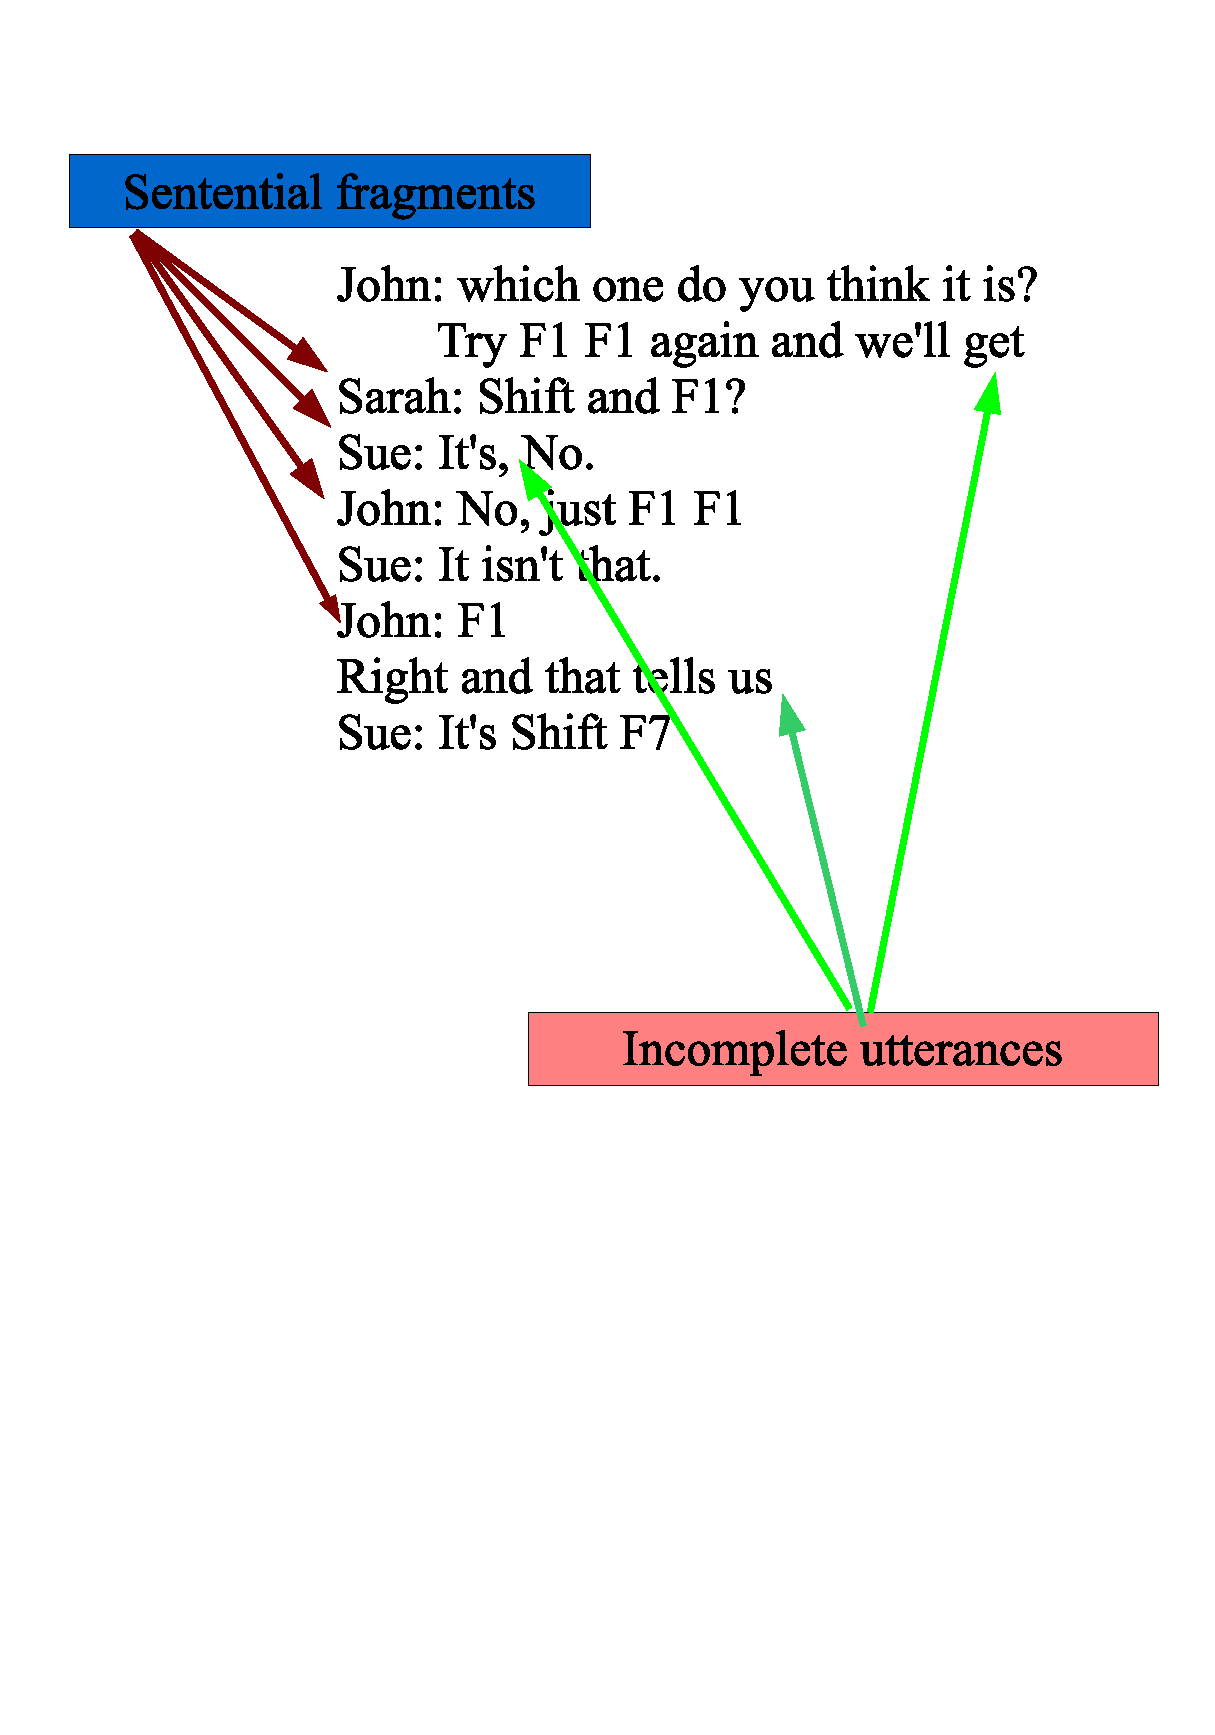
\includegraphics[height=10cm,width=8cm]{challenges0.eps}

%\hfill\hyperlink{SF1}{\beamergotobutton{Back}}
\end{frame}


\begin{frame}\frametitle{Challenges to semantic/discourse theories}

%\begin{figure*}[!h]
%\begin{center}
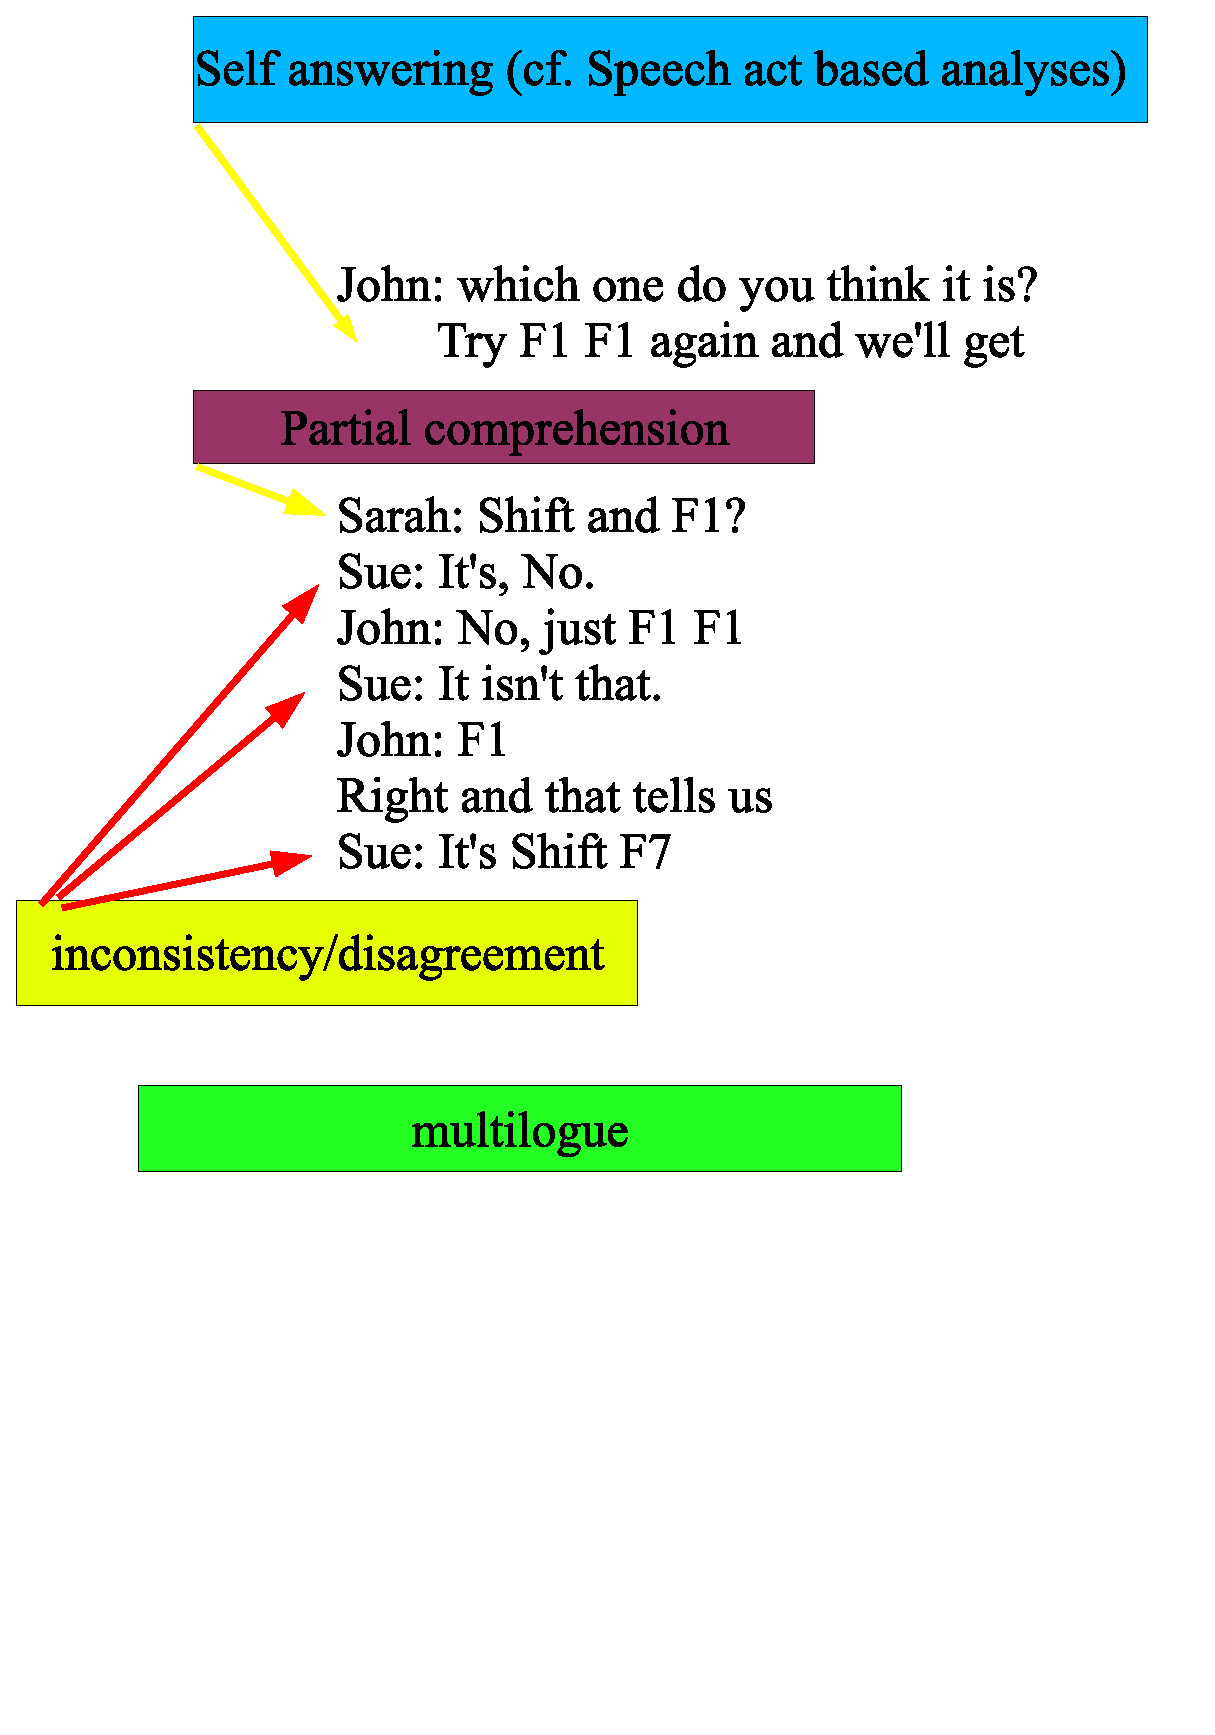
\includegraphics[height=10cm,width=8cm]{challenges1.eps}
%\caption{Sketch of Interrogatives type hierarchy from Ginzburg and Sag 2000} \label{int-hi}
%\end{center}
%\end{figure*}
\end{frame}


\frame{\frametitle{Analyzing the printer example}
\bit

\item NSUs: using DGB-driven context.
\item Dysfluencies using conversation rules of similar form to CRs
  and, more generally, to general conversational rules; requires
  incremental perspective for grammar.
\item Self answering: consequence of QSPEC---factoring turn taking
  from general illocutionary specification.
\item Misunderstanding: accommodated by (i) different DGBs per
  conversational participants, (ii) grounding/CR conditions
  characterized by locutionary propositions (utterance types/tokens)
\item Multilogue involves scaling up of duologue conversational rules;
  main differences: communal grounding/acceptance, turn
  taking,\ldots. (See \cite{gf-acl05,ginzburg-buke})




\eit
}

\frame[allowframebreaks]{\frametitle{ Why Type Theory with Records: Semantic ontology }

\bit

\item Possible worlds semantics has intrinsic problems, ones Montague
  was aware of  when he first used it in his seminal papers in the
  1970s.

\item We saw how TTR provides an ontology which can be used to solve doxastic
  puzzles (propositions) and dialogical puzzles (negation).

\eit
}

\frame[allowframebreaks]{\frametitle{ Why Type Theory with Records:
    Syntax Semantics interface }
\bit
\item We saw how TTR allows one to synthesize $\lambda$-calculus
  driven and unification--based synsem interfaces:

\item Robust meaning/context/content relations
\item GQs
\item Questions
\item Utterance types (for metacommunicative interaction)
\item Frames (for detailed lexical semantics)
\eit
}

\frame{\frametitle{}
{\huge Many Thanks}
}

\bibliographystyle{egapa}
\bibliography{newest-jg-fin}

\end{document}

\ignore{



}

